\documentclass{article}
\usepackage{graphicx}
\usepackage{hyperref}
\usepackage{tcolorbox}
\usepackage{parskip}
\usepackage{enumitem}
\usepackage[authoryear]{natbib}
\usepackage{mdframed}
\usepackage[margin=1in]{geometry}
\usepackage{booktabs}
\usepackage{amsmath}

\title{\textbf{Simon Opsahl}\\AI, Decision Making, and Society\\6.3950/6.3952, Fall 2024\\Pset 6 -- Privacy \& Fairness}

\begin{document}
\date{Due: November 6, 2024 (by 11:59 PM)}

\maketitle

\section*{}

Algorithms are increasingly used to inform or make decisions about our lives in many settings, such as employment, lending, and healthcare. In this problem set, you will explore the privacy and fairness considerations in systems of algorithmic decision-making. This problem set has 4 parts:
\begin{itemize}
    \item Problem 1: Notions of Data Privacy
    \item Problem 2: Differential Privacy \& Unlearning with Census Data
    \item Problem 3: Formal Views of Fairness 
    \item Problem 4: Structural Views of Fairness
\end{itemize}

Note that Problems 1 \& 2 are designed to be completed sequentially, as are Problems 3 \& 4. Please submit your assignment as a PDF compiled from this LaTeX template.

\clearpage
\section*{Problem 1: Notions of Data Privacy}

\textbf{Optional Background Reading:}
\begin{itemize}

\item \href{https://www.whitehouse.gov/ostp/ai-bill-of-rights/data-privacy-2/}{U.S. AI Bill of Rights: Data Privacy}

\item \href{https://www.cis.upenn.edu/~aaroth/Papers/privacybook.pdf}{The Algorithmic Foundations of Differential Privacy} (Dwork and Roth, 2014) (Chapters 1-3)
\item \href{https://salil.seas.harvard.edu/sites/scholar.harvard.edu/files/salil/files/differential_privacy_primer_nontechnical_audience.pdf}{Differential Privacy:
A Primer for a Non-Technical
Audience} (Wood et al. '08) (Pages 225-236, 250-259)
\end{itemize}
\bigskip 

In the context of AI systems, privacy violations are often a repercussion of data-driven decision-making. This problem explores different notions of \textbf{data privacy}.

\subsection*{Privacy Fallacies}

Consider the following fictional scenario: \textit{Some MIT students are writing an in-depth article about a professor named Dylan. Keen to demonstrate their investigative skill, they begin to amass a huge variety of data all about Dylan that they intend to publish in ``The Tech'' newspaper. Since you are a privacy expert, the students consult you about their story.}

\textbf{1. The students from the scenario above make the following claims. Briefly respond to each claim in a few sentences. Answers should refer to material from lecture.}
\begin{enumerate}[label=\Alph*.]
    \item ``Why should Dylan care if we publish this information? If Dylan objects, it must be because they have something to hide!''
    \item ``But many of these records are public anyway! We got them down at the courthouse.''
    \item ``So what if this humiliates Dylan? There aren't any laws to protect embarrassment as a harm.''
\end{enumerate}

\bigskip

\begin{mdframed}
\begin{enumerate}[label=\Alph*.]
\item Dylan may be objecting just because Dylan values their privacy. Just because someone does not want their personal life to be exposed to the world, it does not mean that they have something to hide. Make sure you strike a balance between what is necessary for the story and respecting Dylan's privacy.
\item Dylan's information being publicly accessible is true. When data is available in that way, in general privacy is not violated through obscurity. Just make sure you are careful that what you reveal is legally acquired data.
\item It is true that there aren't really laws to protect against embarrassment. However, if Dylan can prove that you have concretely wronged him and violated his right to be left alone, he may have a case against you. Just make sure that the information that you gather is accurate, legally sourced, and use of any records are justifiable.
\end{enumerate}
\end{mdframed}
\bigskip



\subsection*{Online Data Privacy}

There are many differences between notions of data privacy for offline and online contexts, but a central concern is that online systems collect orders of magnitude more data.  

\textbf{2. The following questions are about data privacy and online platforms (based on US laws). Briefly answer each question in a few sentences. Answers should refer to material from lecture.}
\begin{enumerate}[label=\Alph*.]
\item What is the dead body problem?
\item Why is the accessibility of online information not binary? 
\item Does the first amendment protect against any online speech that infringes privacy? Support your answer with a court case from class.
\item If you post content privately on social media, do you have a reasonable expectation of privacy?
\end{enumerate}

\bigskip

\begin{mdframed}
\begin{enumerate}[label=\Alph*.]
\item The dead body problem refers to the idea that there is a lack of clear evidence that privacy is harmful. Yes, people may be uneasy with their personal information being sold to advertising agencies. The critical point, however, is that there is a lack of severe negative consequences: such as dead bodies.
\item Accessibility of online information is not binary. For example, there are differences between personal information you post on your Facebook vs information you disclose in an email to a friend. There are varying levels of easiness and legality and cost that stratify the accessibility of information.
\item The first amendment does protect against certain infringements on privacy. A good example is Bollea vs. Gawker, where Hulk Hogan sued an online magazine for posting a sex tape taken non-consensually. He won based on the right to be left alone elucidated by Warren and Brandeis. 
\item As long as the information has left your hands and been disclosed to the platform, you likely do not have any defensible case concerning how that data is used. Beyond what companies assure you regarding protection, the information had already in a way been willingly disclosed to a third party. 
\end{enumerate}
\end{mdframed}
\bigskip

\subsection*{Privacy in Datasets}

Many datasets may infringe on the privacy of individuals to varying degrees. For example, datasets used to train AI models and datasets produced by AI systems might contain confidential or personally identifiable information. Even though we can restrict access to these datasets, we may still want to release the outputs of computations over these datasets (e.g. analytical queries or the outputs of AI models). Census data, for instance, has high analytical value, but the release of such aggregated information should protect the privacy of raw individual responses. 

\textbf{3. Recall the video\footnote{\url{https://www.youtube.com/watch?v=pT19VwBAqKA}} that we watched in recitation about protecting privacy in Census data. Answer the following questions based on the video (answers can be short phrases).}
\begin{enumerate}[label=\Alph*.]
\item The video describes an example reconstruction attack based on access to summary statistics of age, gender, and ice cream preferences. What does the output of this attack look like in terms of columns and rows? 
\item What are the x and y axes of the ``plausibilties plot''?
\item What is the tradeoff for privacy?
\item Why can't you just add any old random noise to protect privacy?
\item What is one of the biggest benefits of differential privacy?
\end{enumerate}


\bigskip
\begin{mdframed}
\begin{enumerate}[label=\Alph*.]
\item The reconstruction attack aims to use the released statistics of a column, or feature, to reconstruct the rows, which links an individual to their information.  
\item Plausibility plots graph the relationship between the domain of possible values of a feature (x-axis) against the plausibility of the specific value (y-axis).
\item The trade off for privacy is accuracy of data.
\item Random noise is not sufficient to protect privacy, because when enough results are published with the introduced noise, it is possible to reconstruct the original distribution. 
\item Differential privacy mathematically bounds the privacy loss from releasing some statistic. As a result, you can bound the amount of privacy that is violated over all the information that is released. 
\end{enumerate}
\end{mdframed}
\bigskip


\textbf{4. Even if reconstruction of individual data is not feasible, sometimes even being a member of a dataset is sensitive information. Give two examples of datasets in which membership could be considered sensitive.}
\bigskip
\begin{mdframed}
\begin{itemize}
\item Example 1: Inclusion in a medical study about people suffering from a rare heart disease.
\item Example 2: Participating in a survey about job prospects for closeted LGBTQIA individuals.
\end{itemize}
\end{mdframed}
\bigskip


\subsection*{Randomization for Privacy}

Suppose you’re working with a research group that says they’re using a randomized response protocol to protect privacy of respondents for a yes/no survey question. Their protocol asks the respondent to do the following:
\begin{itemize}
\item With probability 1/3, the respondent should invert their true answer: if their true answer is ``yes'' they should say ``no'', and if their true answer is ``no'' they should say ``yes''.
\item With the remaining 2/3 probability, the respondent should answer truthfully.
\end{itemize}
Let $y$ denote what the researchers want to find: the unknown fraction of the population for whom the true answer is ``yes.'' However, because of the randomized response protocol, they only have access to $q$: the fraction of answers received through the survey that are ``yes.''

\textbf{5. Compute the following quantities (as mathematical expressions). Justify your answers (mathematically).} \textit{If you need help, come to office hours!}
\begin{enumerate}[label=\Alph*.]
\item What is the expected value of $y$ in terms of $q$?
\item What is the probability that a respondent's true answer was ``yes'' given that they responded ``yes'' to the survey? Your answer should be in terms of $y$.
\end{enumerate}

\bigskip
\begin{mdframed}
\begin{enumerate}[label=\Alph*.]
\item We can determine $q$ to be the sum of the contributions from $\frac{2}{3}$ of ``yes" correspondents and $\frac{1}{3}$ of the ``no" correspondents. Thus $q = \frac{2}{3}y + \frac{1}{3}(1-y)$, and $y = 3q - 1$ in expectation.
\item If the true answer is $X$ and the response is $Y$, we are looking for $P(X=1 | Y = 1) = \frac{P(X=1\land Y=1)}{P(Y=1)} = \frac{\frac{2}{3}y}{q} = \frac{\frac{2}{3}y}{\frac{1}{3} + \frac{1}{3}y} = \frac{2y}{1 + y}$.
\end{enumerate}
\end{mdframed}
\bigskip

\textbf{6. You ask the researchers about their use of the number 1/3. ``Actually,'' they say, ``this is the second thing we tried. We started with the same protocol\footnote{Specifically, the protocol that they tried first was as follows: (1) with probability 1/2, the respondent should invert their true answer; (2) with the remaining 1/2 probability, the respondent should answer truthfully.}, but using the number 1/2 instead of 1/3.'' They go on to say: ``a funny thing happened when we tried this original protocol'', but don't elaborate. What did the researchers mean by this?}

\bigskip
\begin{mdframed}
When we calculated the expected value of $y$ from $q$, we used the formula $q = \frac{2}{3}y + \frac{1}{3}(1-y) = \frac{1}{3} + \frac{1}{3}y$. If we replace $\frac{1}{3}$ with $\frac{1}{2}$, this becomes $q = \frac{1}{2}y + \frac{1}{2}(1-y) = \frac{1}{2}$, which means that $q$ does not depend on $y$. As a result, no matter the true proportion $y$, half of all responses will be true and the other half false.
\end{mdframed}
\bigskip


\subsection*{Differential Privacy}

Differential privacy (DP)\footnote{DP was introduced in this \href{https://uvammm.github.io/docs/dwork.pdf}{seminal paper} by Dwork et al. in 2006.} is a formal technique for using randomization to protect the privacy of individuals in a dataset. The main idea behind DP is to ensure that adding or removing any single individual's data to or from the dataset does not significantly affect the outcome of any analysis or ``function'' computed on the data. These computations could range from simple queries on the dataset (like averages or counts) to more complex tasks like training machine learning models. DP achieves privacy by adding carefully calibrated statistical noise to the outputs of these computations, making it difficult to identify any specific individual's data from the output. 

The next few questions walk through the concept of differential privacy using the example dataset of student grades in Table~\ref{tbl:dataset}.

\begin{table}[h!]
    \centering    
    \begin{tabular}{lll}
        \toprule
        \textbf{Student Name} & \textbf{GPA} \\
        \midrule
        Alice             & 3.00 \\
        Ethan             & 3.25 \\
        Naomi             & 3.50 \\
        Liam              & 3.75 \\
        Chloe             & 4.00 \\
        \bottomrule
    \end{tabular}
    \caption{An example dataset of student GPAs (on a scale of 0.0 to 4.0).}
    \label{tbl:dataset}
\end{table}

\textbf{Functions and Output Events}

The formal definition of DP protects privacy for ``functions'' $f$ computed over the data. For example, average GPA is a function that could be computed over student grades. The definition also relies on the concept of \textbf{output events} $T \in \text{Range}(f)$, where $\text{Range}(f)$ is the possible outputs of the function $f$. In other words, an output event could be a single possible value, or a range of values, that a function could take. 

\textbf{7. Answer the following questions about functions and output events based on Table~\ref{tbl:dataset}.}
\begin{enumerate}[label=\Alph*.]
\item Suppose $f$ is average GPA. What is $f(\mathcal{D})$, where $\mathcal{D}$ is the dataset in Table 1?
\item Suppose no noise is added to output of $f$. What is the probability that $f(\mathcal{D}) \in T$, where $T = [3.0, 3.25]$?
\item Suppose noise drawn uniformly from the range $[-0.5,0.5]$ is added to the output of $f$. What is the probability that $f(\mathcal{D}) \in T$, now that $f$ includes the added noise?
\end{enumerate}

\bigskip
\begin{mdframed}
\begin{enumerate}[label=\Alph*.]
\item The average GPA from Table 1 is 3.5.
\item With the addition of no noise, the probability that $f(\mathcal{D})\in T$ is 0 because the true value lies outside the range. 
\item If the true value of the population mean is 3.5, and we are adding noise from the uniform distribution $\epsilon \in [-0.5, 0.5]$, then $f(\mathcal{D}) +\epsilon$ is also a uniform distribution ranging from 3 to 4. The likelihood that the $f(\mathcal{D}) +\epsilon \in T = \frac{\text{range}{(T)}}{\text{range}(\epsilon)}= \frac{0.25}{1} = 0.25 $.
\end{enumerate}
\end{mdframed}
\bigskip

\textbf{Neighboring Datasets}

The formal definition of DP further relies on the concept of neighboring datasets. Two datasets $\mathcal{D}$ and $\mathcal{D}'$ are neighbors if and only if they differ in the \underline{inclusion or exclusion} of one data point (e.g. the data for one individual).

\textbf{8. Answer the following questions about neighboring datasets based on Table~\ref{tbl:dataset}.}
\begin{enumerate}[label=\Alph*.]
\item Describe an example of a neighboring dataset in this scenario.
\item What is the difference in average GPA between the original table and the table without Ethan?
\item What is the maximal difference in average GPA between the original table and \underline{any} neighboring dataset?
\end{enumerate}

\bigskip
\begin{mdframed}
\begin{enumerate}[label=\Alph*.]
\item An example of a neighboring dataset would be all of the data in Table 1 with the addition of another row: Jeremy with a GPA of 4.00.
\item When we don't include Ethan in calculating the average GPA, the new average is 3.5625. The difference is 0.0625.
\item The maximal difference would come from including a student with a GPA of 0.00 in $\mathcal{D}'$. The new average is 2.9167, which is a difference of 0.5833.
\end{enumerate}
\end{mdframed}
\bigskip

\textbf{Noise Mechanism}

The high-level idea behind DP is that the noise needed to protect privacy depends on the maximal difference between outputs of $f$ across neighboring datasets (as you analyzed in 8B). This problem set omits the details, although graduate students will explore a specific noise mechanism in Question 11.

\textbf{9. Suppose $f(\mathcal{D})$ is the average GPA of $\mathcal{D}$, where $\mathcal{D}$ is the dataset in Table~\ref{tbl:dataset}, but now we are adding some noise $z$.}
\begin{enumerate}[label=\Alph*.]
\item Suppose $\mathcal{D}'$ is $\mathcal{D}$  without Ethan. What should $z_1 - z_2$ be so that $f(\mathcal{D}) + z_1 = f(\mathcal{D'}) + z_2$?
\item Suppose $\mathcal{D'}$ is the neighboring dataset with the farthest average GPA from Table 1. What should $z_1 - z_2$ be so that $f(\mathcal{D}) + z_1 = f(\mathcal{D'}) + z_2$?
\end{enumerate}

\bigskip
\begin{mdframed}
\begin{enumerate}[label=\Alph*.]
\item If $f(\mathcal{D}) + z_1 = f(\mathcal{D'}) + z_2$, then $z_1 - z_2 = f(\mathcal{D'}) - f(\mathcal{D}) = 3.5625 - 3.5 = 0.0625$.
\item If $f(\mathcal{D}) + z_1 = f(\mathcal{D'}) + z_2$, then $z_1 - z_2 = f(\mathcal{D'}) - f(\mathcal{D}) = 2.9167 - 3.5 = -0.5833$.
\end{enumerate}
\end{mdframed}
\bigskip



\textbf{Formal Guarantee}

The formal guarantee provided by an $\epsilon$-differentially private noise mechanism is as follows. For a given $\epsilon>0$, the function $f$ satisfies differential privacy if, for all pairs of neighboring datasets $\mathcal{D}$ and $\mathcal{D}'$, and all output events $T \in \text{Range}(f)$:

\begin{align*}
    \label{eq:DP_Def}
    P(f(\mathcal{D}) \in T) \leq e^{\epsilon} \cdot P(f(\mathcal{D}') \in T)
\end{align*}

Informally, this definition can be understood as ``the results of the function $f$ when applied to any neighboring datasets $\mathcal{D}$ and $\mathcal{D}'$ are close to each other, in a way that an external observer cannot distinguish between them.'' The parameter $\epsilon$ quantifies the privacy of the algorithm, as a bound on the maximum amount by which the inclusion or exclusion of a single data point can affect the results.

\textbf{10. Answer the following questions about the formal guarantee provided by differential privacy, based on $\mathcal{D}$ being the dataset in Table~\ref{tbl:dataset}}.
\begin{enumerate}[label=\Alph*.]
\item Suppose once again that $f$ is average GPA, and that no noise is added to $f$. If $T = 3.50$, does $f$ satisfy differential privacy for any $\epsilon$?
\item Suppose $\epsilon_1 > \epsilon_2$. Which $\epsilon$ provides more privacy? Which requires more noise to be added, on average? 
\end{enumerate}

\bigskip
\begin{mdframed}
\begin{enumerate}[label=\Alph*.]
\item If $T= 3.50$, then the probability that $P(f(\mathcal{D}) \in T)=1$, and no $\epsilon >0$ satisfies differential privacy, as there are some $\mathcal{D'}$ where $P(f(\mathcal{D'}) \in T) = 0$.
\item $\epsilon_2$ provides more privacy because the upper bound on the $P(f(\mathcal{D}) \in T)$ is tighter. With the same logic, $\epsilon_2$ requires more noise in order to abide by these bounds.
\end{enumerate}
\end{mdframed}
\bigskip


\subsection*{Additional exercise for students in 6.3952}

\textit{This question is only required for students enrolled in the graduate version of the class.}

The Laplace mechanism is one way to add noise to satisfy differential privacy. Specifically, for any $f : \mathcal{D} \mapsto \mathcal{R}$, the Laplace mechanism outputs: $$f(\mathcal{D}) + \text{Lap}(\Delta f / \epsilon)$$ where $\Delta f$ is the maximum difference in $f$ between $\mathcal{D}$ and any neighboring dataset:
$$\Delta f = \max_{\mathcal{D}, \mathcal{D}'} |f(\mathcal{D}) - f(\mathcal{D}')|$$

and $\text{Lap}(b)$ is a random draw from a Laplace random variable with mean 0 and scale parameter $b$. The probability density function of the Laplace distribution with mean 0 and scale parameter $b$ is given by:
$$p(z \, | \, 0, b) = \frac{1}{2b} \cdot \exp \left(-\frac{|z|}{b}\right)$$.

\textbf{11. Prove that the Laplace mechanism satisfies $\epsilon$-DP. Specifically, prove that the following expression is true for any output event $T \in \text{Range}(f)$:} $$\frac{P\,[f(\mathcal{D}) + \text{Lap}(\Delta f / \epsilon) = T ]}{P\,[f(\mathcal{D'}) + \text{Lap}(\Delta f / \epsilon)= T]} \leq e^\epsilon$$

\textit{Hint: To simplify, you will need the reverse triangle inequality: $| |a| - |b| | \leq |a - b|$, where $a$ is $|T-f(\mathcal{D}')|$ and $b$ is $|T-f(\mathcal{D})|$.}

\bigskip
\begin{mdframed}
When we look at the probability, $$P\,[f(\mathcal{D'}) + \text{Lap}(\Delta f / \epsilon)= T]$$we can rewrite it as $$P\,[\text{Lap}(\Delta f / \epsilon)= T - f(\mathcal{D'})]$$which can evaluated via the probability density function with a $b = \Delta f/\epsilon$ and $z = T - f(\mathcal{D'})$. It thus becomes
$$\frac{\epsilon}{2\Delta f} \cdot \exp \left(-\frac{|T - f(\mathcal{D'})| \cdot \epsilon}{\Delta f}\right)$$

We can thus transform the below expression as 
$$\frac{P\,[f(\mathcal{D}) + \text{Lap}(\Delta f / \epsilon) = T ]}{P\,[f(\mathcal{D'}) + \text{Lap}(\Delta f / \epsilon)= T]} = \frac{\frac{\epsilon}{2\Delta f} \cdot \exp \left(-\frac{|T - f(\mathcal{D})| \cdot \epsilon}{\Delta f}\right)}{\frac{\epsilon}{2\Delta f} \cdot \exp \left(-\frac{|T - f(\mathcal{D'})| \cdot \epsilon}{\Delta f}\right)} = \exp \left(\frac{\epsilon}{\Delta f} \cdot (|T - f(\mathcal{D'})| - |T - f(\mathcal{D})|)  \right)$$

In this problem, we rely on the fact that $$|f(\mathcal{D}) - f(\mathcal{D'})| \leq \Delta f$$
We can expand this and use the triangle inequality to establish $$| |T - f(\mathcal{D'})| - |T-f(\mathcal{D})| | \leq|(T - f(\mathcal{D'})) - (T-f(\mathcal{D}))| \leq \Delta f$$

We can use this to upper bound the above expression as $$\exp \left( \frac{\epsilon}{\Delta f} \cdot \Delta f\right) = e^{\epsilon}$$

As a result, we have proven that 
$$\frac{P\,[f(\mathcal{D}) + \text{Lap}(\Delta f / \epsilon) = T ]}{P\,[f(\mathcal{D'}) + \text{Lap}(\Delta f / \epsilon)= T]} \leq e^\epsilon$$
\end{mdframed}
\bigskip


\clearpage
\section*{Problem 2: Differential Privacy \& Unlearning with Census Data}
\textit{Note: This problem will directly build on the activity in Recitation 7 on 10/25. You may want to wait until after recitation to begin this problem.}

\bigskip 
\textbf{Optional Background Reading:}
\begin{itemize}

\item \href{https://www2.census.gov/library/publications/decennial/2020/census-briefs/c2020br-03.pdf}{Why the Census Bureau Chose
Differential Privacy} (2020 Census Briefs)

\item \href{https://privacytools.seas.harvard.edu/blog/differential-privacy-2020-census-how-can-we-make-data-both-private-and-useful}{Differential Privacy for the 2020 Census} (Gong et al. 2022)

\item \href{https://arxiv.org/pdf/1610.05820}{Membership Inference Attacks Against Machine Learning Models} (Shokri et al. 2017)

\item \href{https://arxiv.org/pdf/2209.12269}{Algorithms that Approximate Data Removal} (Suriyakumar \& Wilson, 2022)

\end{itemize}
\bigskip 

As you explored in Problem 1, differential privacy (DP) is a fundamental technique for protecting individual records in datasets.  Recall that the formal guarantee provided by an $\epsilon$-differentially private noise mechanism is as follows. For a given $\epsilon>0$, the function $f$ satisfies differential privacy if, for all pairs of neighboring datasets $\mathcal{D}$ and $\mathcal{D}'$, and all output events $T \in \text{Range}(f)$:

\begin{align*}
    P(f(\mathcal{D}) \in T) \leq e^{\epsilon} \cdot P(f(\mathcal{D}') \in T)
\end{align*}

This problem builds upon the activity in Recitation 7, where we compared classifiers trained with and without DP on the Iris dataset and assessed their resilience to database reconstruction tasks. However, in this problem, we will apply differential privacy to the \href{https://archive.ics.uci.edu/dataset/2/adult}{Census Adult dataset}, and test resilience to a different type of attack: membership inference. We will also briefly explore the concept of unlearning, which is another way to ensure the privacy of individual records in datasets. 

To complete this exercise, you will need to make a copy of this \href{https://colab.research.google.com/drive/1Q1TWMmQLQb0pmez9p5RFQHJtJKEwBeuM?usp=sharing}{Colab Notebook} and fill in some sections. However, you will only need the Colab for certain parts below, and you will provide all your answers in this LaTeX document.


\subsection*{Exploratory Data Analysis}

In this problem, we will use the \href{https://archive.ics.uci.edu/dataset/2/adult}{Census Adult dataset}, which contains demographic data about individuals across the US. One goal from using this dataset is to be able to predict whether or not the annual income of an individual exceeds \$50K/yr. Please upload the files ``adult.data" and ``adult.test" to your colab before starting the exercise. 

\textbf{1. In the notebook, run the cells in the ``Exploratory Data Analysis'' section (you do not need to change any code, just analyze the visualizations). Then, answer the following questions.}
\begin{enumerate}[label=\Alph*.]
\item Based on the visualization of income and highest-level of education, which education levels have more individuals earning over \$50K compared to those earning \$50K or less?
\item Based on the visualization of income and gender, roughly what percentage of women earn over \$50K?
\item Based on the histogram of age, what is the shape of the distribution? Why is it shaped this way?
\item Based on the histogram for hours worked for week, what is the shape of the distribution? Why is it shaped this way? 
\end{enumerate}

\bigskip

\begin{mdframed}
\begin{enumerate}[label=\Alph*.]
\item The education levels that have more individuals earning over \$50K than not are Masters, Doctorate, and Professional Schools.
\item Roughly 10\% of women earn over \$50K based on the visualization.
\item The plot is right skewed with a mode in between 30 and 40. Differences in counts by generation occur because of different trends of having children and other context-dependent things at different times.
\item The distribution is roughly symmetric with a sizable mode around 40 hours a week. This is due to the convention of the American 40 hr work week.
\end{enumerate}
\end{mdframed}

\bigskip


\subsection*{Building Models with DP}

Our goal is to build a differentially-private classifier of whether a person's annual income is greater or less than \$50K. For our implementation, we will use a \textbf{logistic regression} classifier. For logistic regression\footnote{For additional background, see this paper by \href{https://systems.cs.columbia.edu/private-systems-class/papers/Chaudhuri2009Privacy.pdf}{Chaudhuri et al.}}, differential privacy can be achieved by adding carefully calibrated noise to the learned vector of weights $\theta$. The noise helps protect individual data points from being identified, while still keeping the model accuracy similar to the original model. Recall that logistic regression finds a vector $\theta$ such that, given a vector of features $x_i$, the model estimates the probability of $y_i = 1$ as follows:
\begin{align}
    P(y_i = 1|x_i) = \frac{1}{1 + e^{-2\theta^{T}x_i}}
\end{align}

\textbf{In the notebook, run the code in the ``Building Models with DP'' section to answer the following questions.}

\textbf{2. The following questions are based on the cell that asks you to try different $\epsilon$. Report accuracy to 5 decimal places.}

\begin{enumerate}[label=\Alph*.]
    \item What is the accuracy of the baseline model without DP?
    \item What is the accuracy of the model with $\epsilon=0.01$?
    \item What is the accuracy of the model with $\epsilon=0.1$?
    \item What is the accuracy of the model with $\epsilon=1.0$?
    \item As $\epsilon$ increases, will the accuracy ``increase'', ``decrease'', or ``stay the same'' on average? Briefly justify your answer.
\end{enumerate}


\bigskip
\begin{mdframed}
\begin{enumerate}[label=\Alph*.]
    \item The baseline accuracy is 0.82039.
    \item When $\epsilon = 0.01$, the accuracy is 0.65137.
    \item When $\epsilon = 0.1$, the accuracy is 0.73928.
    \item When $\epsilon = 1.0$, the accuracy is 0.81834.
    \item When we increase $\epsilon$, the accuracy will tend to increase, and that is because we have looser bounds with the higher $\epsilon$, and thus less noise needs to be added.
\end{enumerate}
\end{mdframed}
\bigskip

\textbf{3. The following questions are based on the visualization of accuracy and different $\epsilon$.}

\begin{enumerate}[label=\Alph*.]
    \item For what $\epsilon$ are the model predictions essentially a random guess?
    \item For what $\epsilon$ does the accuracy match the baseline model without DP?
    \item Your curve may have some fluctuations (e.g. it is not smooth). In general, why would we expect this to be the case?
    \item How would you recommend that a real-world deployment choose $\epsilon$? What are the trade-offs?
\end{enumerate}

\bigskip
\begin{mdframed}
\begin{enumerate}[label=\Alph*.]
    \item For $\epsilon < 0.01$, the accuracy is instable around 0.5 and thus is essentially a random guess.  
    \item For $\epsilon > 1$, the accuracy is roughly equivalent to the baseline.
    \item The curve is not smooth because we are dealing with non-deterministic systems, and the introduction of noise also leads to a random element contributing to the accuracy. 
    \item A real-world deployment would need to establish thresholds for both accuracy and privacy that they would like to maintain, and search through the space of epsilons until they find one that sufficiently satisfies both. Increasing privacy decreases accuracy, and vice versa, so the choice must be deliberate.
\end{enumerate}
\end{mdframed}


\subsection*{Membership Inference Attacks}



The goal of differential privacy is often to protect against adversarial attacks that may be able to glean some sensitive information about the dataset. One type of attacks are \textbf{membership inference attacks} (MIA), which aim to determine whether a specific data point (e.g. an individual) is in a dataset.

For our setting, consider the salary prediction model that we have trained using the Census data. An adversary may want to know whether a particular individual was included in the training data used for this model. In this case, the salary prediction model that we have built is the ``target model.'' The adversary's goal is to build an ``attack model'' which tries to infer whether a data point was included in the training set of the ``target model''. In order to do this, the adversary needs access to some information from the target model, such as its predictions. For our setting, we make two assumptions:
\begin{itemize}
    \item Assumption 1: The adversary can make unlimited queries to the target model, and thus collect predictions for many data points. 
    \item Assumption 2: The adversary has access to a subset\footnote{In our implementation, we make the stronger assumption that the adversary knows a subset of data points in the training set and a subset of data points not in the training set, and that these subsets have data points that are sufficiently different.} of the training data (i.e. it knows the membership status of some data points).
\end{itemize}

\begin{figure}[h!]
\centering
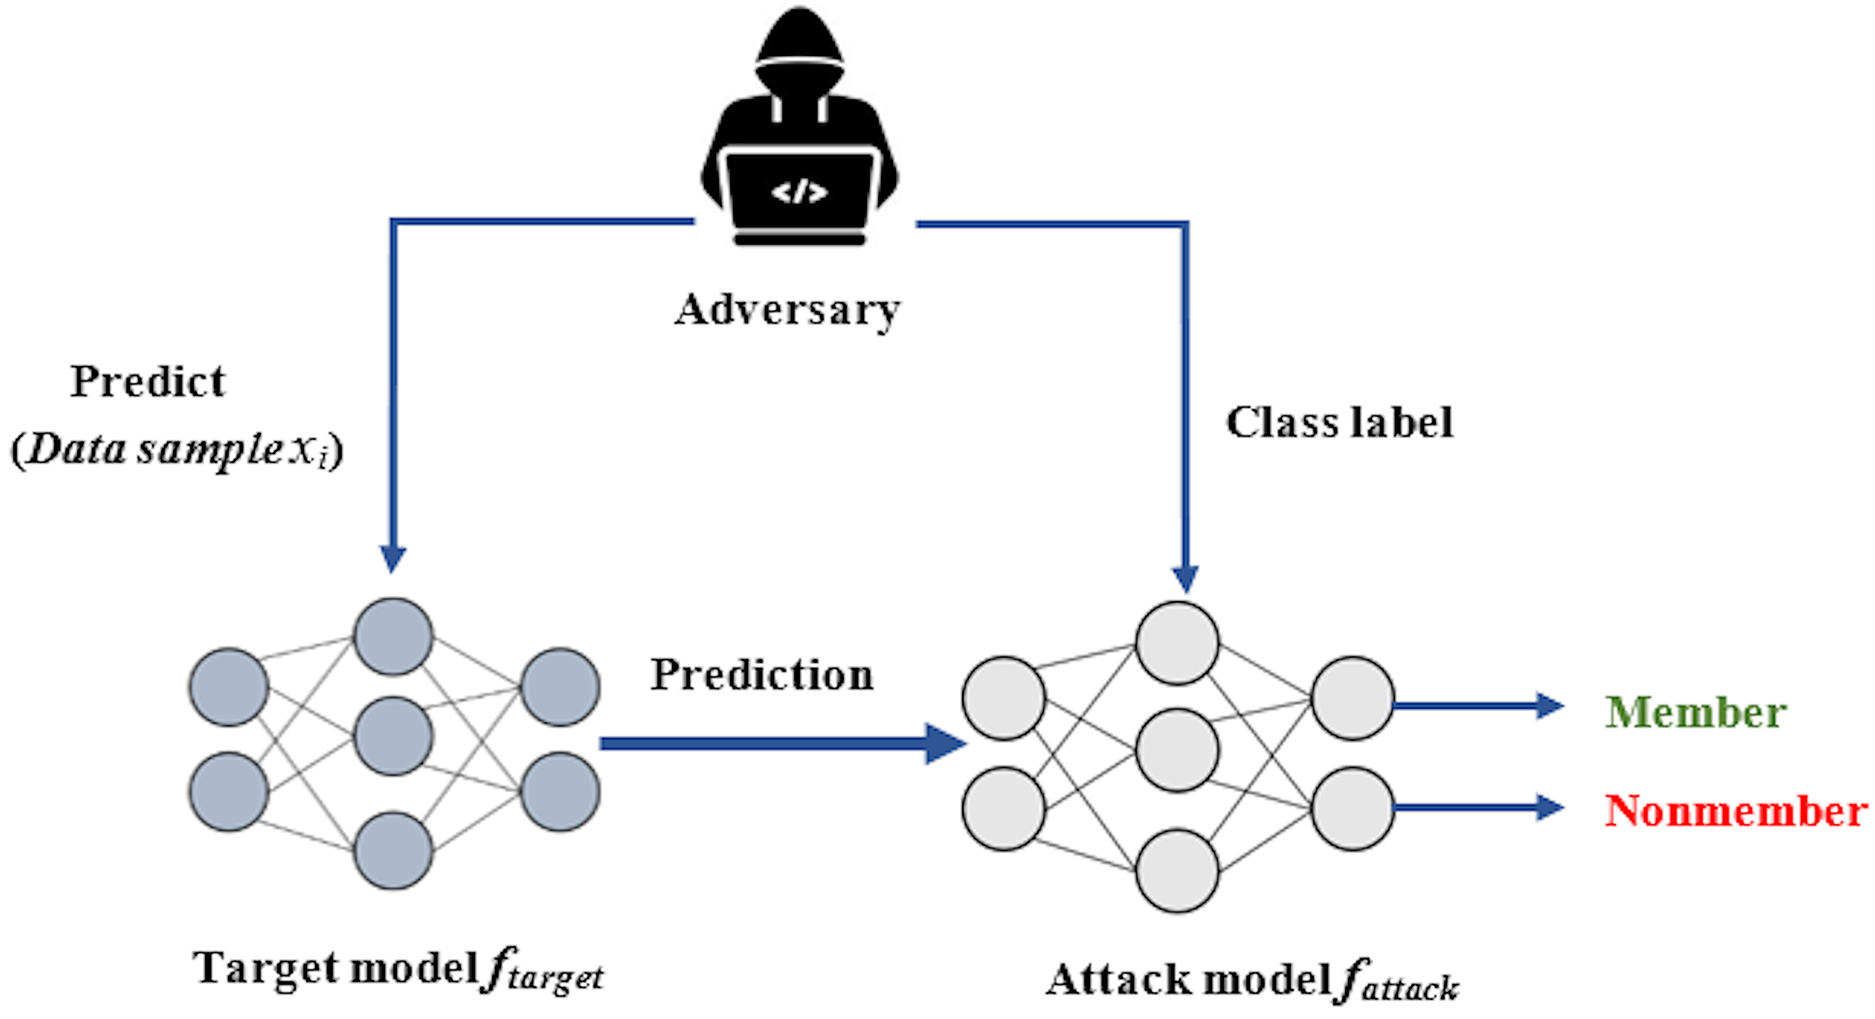
\includegraphics[width=0.5\columnwidth]{MIA.png}
\caption{Membership inference attack: the adversary uses the target model's outputs to determine if a specific data point was a member of the training set.}
\label{fig:MIA}
\end{figure}


\textbf{4. In the notebook, use the code in the ``Membership Inference Attack'' section to answer the following questions. The code will report the accuracy of the attack model (i.e. how well it can determine if a point was in the training set). Report accuracy to 5 decimal places. Note that due to the noise in the process, you might see fluctuations in your results. }

\begin{enumerate}[label=\Alph*.]
    \item What is the attack model accuracy for a model trained with $\epsilon=0.001$?
    \item What is the attack model accuracy for a model trained with $\epsilon=0.01$?
    \item What is the attack model accuracy for a model trained with $\epsilon=0.1$?
    \item What is the attack model accuracy for a model trained with $\epsilon=1.0$?
    \item As $\epsilon$ increases, will the attack model accuracy ``increase'', ``decrease'', or ``stay the same'' on average? Briefly justify your answer, and compare it to your answer in 2(E).
\end{enumerate}

\bigskip
\begin{mdframed}
\begin{enumerate}[label=\Alph*.]
    \item When $\epsilon = 0.001$, the attack model accuracy is 0.53592.
    \item When $\epsilon = 0.01$, the attack model accuracy is 0.57615.
    \item When $\epsilon = 0.1$, the attack model accuracy is 0.65409.
    \item When $\epsilon = 1.0$, the attack model accuracy is 0.71709.
    \item As $\epsilon$ increases, the attack model accuracy also increases. This is the same phenomena encountered in 2(E). This is a result of the fact that higher $\epsilon$ means looser bounds, and thus less noise is added to the data.
\end{enumerate}
\end{mdframed}

\subsection*{Unlearning}

So far, this problem set has focused on differential privacy as a way to protect against membership inference attacks. But if we know certain individuals might be at risk, another approach might be to have the model ``unlearn'' these training examples. 

Unlearning involves taking a trained model and removing the influence of certain training examples (dubbed the ``forget set''). Due to computational limitations, unlearning is often more practical than re-training a model from scratch without the ``forget set''. However, the goal is to make the ``unlearned'' model as close as possible to the model that could be re-trained from scratch. This process is illustrated in Figure ~\ref{fig:Unlearning}. 

\begin{figure}[h!]
\centering
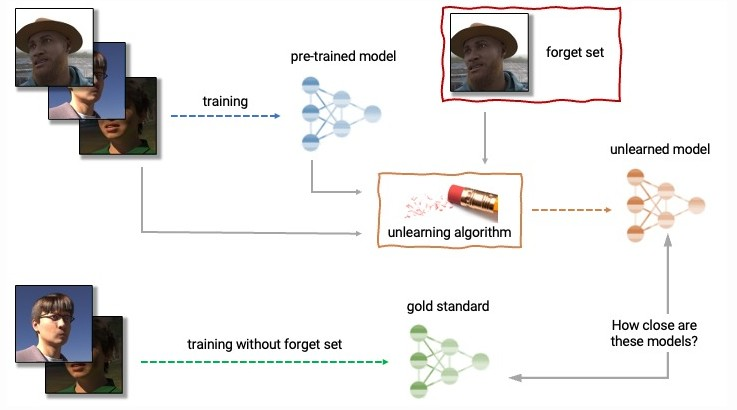
\includegraphics[width=0.75\columnwidth]{Unlearning.jpg}
\caption{An overview of how models ``unlearn'' training samples.}
\label{fig:Unlearning}
\end{figure}

In this exercise, you will test a simple unlearning algorithm that continues training the model on a subset of the training set that excludes the ``forget set'' (also known as the ``retain set''). You will then test the performance of the membership inference attack to check if unlearned samples are \textit{indistinguishable} from samples that were not in the training set. Specifically, the notebook will report the accuracy of the membership inference attack on the forget set and samples not from the training set (this accuracy should be around 50\%, if the unlearning algorithm is successful). 


\textbf{5. In the notebook, run the code in the ``Unlearning'' section to answer the following questions. You do not need to change any of the code in this section, apart from choosing the number of samples to unlearn.}

\begin{enumerate}[label=\Alph*.]
    \item After unlearning 500 training examples, what is the accuracy of the membership inference attack? 
    \item After unlearning 5000 training examples, what is the accuracy of the membership inference attack?
    \item As the number of samples to unlearn increases, will the accuracy of the membership inference attack ``increase'', ``decrease'', or ``stay the same''? Briefly justify your answer.
\end{enumerate}

\bigskip
\begin{mdframed}
\begin{enumerate}[label=\Alph*.]
    \item With 500 unlearned training examples, the membership inference attack accuracy is 0.68.
    \item With 5000 unlearned training examples, the membership inference attack accuracy is 0.78.
    \item As the number of samples to unlearn increases, the accuracy of the attack increases, because the effectiveness of unlearning while maintaining accuracy diminishes as the number of samples increase because of diminishing returns. 
\end{enumerate}
\end{mdframed}

\subsection*{Differential Privacy and Governance}

Differential privacy is often highlighted in governance discussions around AI and privacy, as you will explore in the following reflection questions. Your responses can be brief (a few sentences for each part).

\textbf{6. The following questions are based on \href{https://simons.berkeley.edu/news/differential-privacy-issues-policymakers}{this article} discussing DP and issues for policymakers. Read the article, then answer the following questions.}
\begin{enumerate}[label=\Alph*.]
    \item Why does the article claim the trade-off between privacy and accuracy is not straightforward?
    \item What are ``linking attacks''? Why do they pose a challenge for legal requirements about privacy?
    \item The article claims that ``any deployment of differential privacy requires a value judgment.'' What does this mean? Provide an example based on the Census.
\end{enumerate}

\bigskip
\begin{mdframed}
\begin{enumerate}[label=\Alph*.]
    \item The trade off between privacy and accuracy is not straightforward because there are methods of encryption that occur before centralization of data that further protect privacy. There also is growing research into techniques that improve both acuracy and privacy.
    \item A linking attack is when some adversary connects data that they possess with released data to deanonymise the results. They pose a challenge for current privacy requirements because a lot of identifying information (SSN, address, name, etc.) is publicly available. Many laws only restrict publishing info that can be directly connected to an individual, but because of the vast corpus of information availble, adversaries can combine their sources.
    \item The value judgment is necessary because the importance of valuing privacy or accuracy more depends on the context. For the Census, there are two trains of thought. Firstly, privacy is important because the data collected during the Census is very personal. Conversely, the type of analysis usually performed on census data requires high accuracy because it is dependent on outliers, on notable points, on local trends. The value judgment concerns deciding which viewpoint holds precedence.
\end{enumerate}
\end{mdframed}
\bigskip


\textbf{7. The following questions are based on the recent \href{https://www.whitehouse.gov/briefing-room/presidential-actions/2023/10/30/executive-order-on-the-safe-secure-and-trustworthy-development-and-use-of-artificial-intelligence/} {U.S. executive order} on the ``Safe, Secure, and Trustworthy Development and Use of Artificial Intelligence''. You do not need to read the entire E.O. -- simply refer to the specified sections.}
\begin{enumerate}[label=\Alph*.]
    \item Refer to section 2(f), which starts with ``Americans’ privacy and civil liberties must be protected as AI continues advancing.'' Which constitutional amendment is mentioned? Could a different amendment have been included?
    \item Refer to section 3(z), which provides a definition for ``privacy-enhancing technology.'' The definition mentions several methods other than DP. Choose 2 methods and describe\footnote{If you are unfamiliar with these methods, you may look them up using any online resource of your choice.} each in your own words.
    \item Refer to section 9, which is titled ``Protecting Privacy.'' The section instructs the federal government to create guidelines about DP. What will the guidelines cover?
\end{enumerate}

\bigskip
\begin{mdframed}
\begin{enumerate}[label=\Alph*.]
    \item Section 2(f) discusses the impact of privacy on First Amendment rights. They could also consider the Fourth Amendment and the impact on the right to be left alone.
    \item Homomorphic encryption allows for computation on encrypted data without the need for decryption beforehand. As a result, users can rely on their data not being accessible to \textbf{anyone} but themselves. Zero-knowledge proofs concern the communication of some fact without any accompanying information.
    \item Section 9 instructs the government to identify commercially available information and review current policies concerning it. It also instructs the government to invest in strategies and research protecting against privacy risk.
\end{enumerate}
\end{mdframed}
\bigskip

\textbf{8. The following questions are based on the National Institute of Standards and Technology (NIST)
\href{https://nvlpubs.nist.gov/nistpubs/SpecialPublications/NIST.SP.800-226.ipd.pdf}{guidelines} for DP that came out of the E.O. Read section 3.3 about bias (pages 23-26), then answer the following questions.}


\begin{enumerate}[label=\Alph*.]
\item How can differential privacy magnify disparate impacts on small groups? Describe the examples in Figures 10 and 11.
\item In the context of differential privacy, how does the document distinguish between systemic bias, human bias, and statistical bias?
\end{enumerate}

\bigskip
\begin{mdframed}
\begin{enumerate}[label=\Alph*.]
    \item Small groups are more affected by differential privacy because of the impact of noise. Because smaller groups have less data adding significant noise allows for the possibility of complete erasure, as seen by the error bars of the American Indian population. It also means that downstream accuracy is worse because of the higher variance, as seen by the difference in classifier accuracy for the majority race and minority races.
    \item The document defines systemic bias in differential privacy as the disparate accuracy and magnitude impact on smaller subpopulations of the data. Human bias in this context is the lack of respect of the validity of the results of differential privacy because of the addition of noise. Lastly, statistical bias can be present in post-processing of data or results to make it appear more like ``good data".
\end{enumerate}
\end{mdframed}
\bigskip



\clearpage
\section*{Problem 3: Formal Views of Fairness}

\textbf{Optional Background Reading}:
\begin{itemize}
    \item \href{https://www.propublica.org/article/machine-bias-risk-assessments-in-criminal-sentencing}{Machine Bias (ProPublica 2016)}
    \item \href{https://www.documentcloud.org/documents/2998391-ProPublica-Commentary-Final-070616.html}{COMPAS Risk Scales: Demonstrating Accuracy Equity and Predictive Parity (Northpointe, 2016)}
    \item \href{https://www.propublica.org/article/technical-response-to-northpointe}{Technical Response to Northpointe (ProPublica 2016)}
    \item \href{https://arxiv.org/pdf/1609.05807}{Inherent Trade-Offs in the Fair Determination of Risk Scores (Kleinberg, Mullainathan, and Raghavan 2016)}
\end{itemize}

This problem explores formal views of algorithmic fairness through an analysis of the COMPAS risk assessment tool. COMPAS (``Correctional Offender Management Profiling for Alternative Sanctions'') is a risk assessment tool used in the criminal justice system to predict the likelihood of a defendant re-offending (recidivism). The algorithm is proprietary, but it is based on a questionnaire of 137 items covering personal background, criminal history, and psychological factors. 

In this problem, you will explore how different formal notions of fairness\footnote{COMPAS is based on the assumption that pretrial detention of some individuals is acceptable. However, many argue that most defendants should be released on their own recognizance since they haven't been convicted. Even modest bail requirements can disproportionately burden vulnerable populations. While some jurisdictions have reformed the pretrial process by ending cash bail, pretrial detention remains common.} through a sample of COMPAS risk scores for defendants from Broward County, Florida. To complete this exercise, you will need to make a copy of \href{https://colab.research.google.com/drive/1_dyhl8robpqxn6r0JQ2D87TuZS4x1k7w?usp=sharing}{this Colab Notebook} and fill in some sections. However, you will only need the Colab for certain parts below, and you will provide all your answers in this LaTeX document. 


\subsection*{Background}

In 2016, ProPublica published a now-famous \href{https://www.propublica.org/article/machine-bias-risk-assessments-in-criminal-sentencing}{article} that criticized COMPAS for racial bias. In particular, they argued that the algorithm exhibited a higher false positive rate for black defendants and a higher false negative rate for white defendants. \href{https://www.documentcloud.org/documents/2998391-ProPublica-Commentary-Final-070616.html}{Northpointe} (the makers of COMPAS, now re-branded as Equivant) argued that the algorithm does not use race information and that it is calibrated across racial groups. Both analyses were based on a ``ground-truth'' label of two-year recidivism (i.e. whether or not the defendant re-offended in two-years).

\textbf{1. COMPAS risk scores are often presented to judges as deciles, or on a scale of 1 to 10, where higher scores indicate a greater likelihood of recidivism. Based on the respective claims by ProPublica and Northpointe, answer the following questions.}
\begin{enumerate}[label=\Alph*.]
\item Among defendants that did not recidivate, who did ProPublica claim had higher COMPAS risk scores: black or white defendants?
\item Among re-offending defendants, who did ProPublica claim had lower COMPAS risk scores: black or white defendants?
\item Based on Northpointe's claim that COMPAS is calibrated\footnote{Recall the definition of calibration from lecture, or read the definition provided for question 5 in this problem.} within groups, who should have a higher recidivism rate: black defendants in the 2nd decile, or white defendants in the 2nd decile?
\end{enumerate}

\bigskip
\begin{mdframed}
\begin{enumerate}[label=\Alph*.]
\item ProPublica claimed that black defendants had a higher COMPAS risk score among the set of defendants who did not recidivate. 
\item ProPublica claimed that white defendants had a lower COMPAS risk score among the set of defendants who did recidivate.
\item Assuming that COMPAS is calibrated within groups, black and white defendants in the 2nd decile should both have around a 20\% recidivism rate. 
\end{enumerate}
\end{mdframed}
\bigskip

\textbf{2. In the notebook, run the ``Setup'' cell and complete the code in the ``Exploratory Data Analysis'' section. Then, answer the following questions.}
\begin{enumerate}[label=\Alph*.]
\item Using the histogram of COMPAS deciles by defendant race, which deciles have more white defendants than black defendants?
\item How does the distribution of defendants by decile differ for white defendants and black defendants?
\item What is the two-year recidivism rate (base rate) for white defendants?
\item What is the two-year recidivism rate (base rate) for black defendants?
\end{enumerate}

\bigskip
\begin{mdframed}
\begin{enumerate}[label=\Alph*.]
\item Only a decile of 1 has a higher count of white defendants.
\item The distribution of defendants is very left skewed for white defendants, whereas for black defendants it is roughly uniform across all of the deciles.
\item The base rate of two-year recidivism for white defendants is 39\%.
\item The base rate of two-year recidivism for black defendants is 52\%.
\end{enumerate}
\end{mdframed}
\bigskip

\textbf{3. The following questions are about recidivism predictors in general (not strictly COMPAS). Answer each in a short paragraph.}
\begin{enumerate}[label=\Alph*.]
\item If black defendants have a higher recidivism rate than white defendants, do you think risk scores for recidivism should be higher for black defendants on average? Why or why not?
\item Describe at least two potential sources of bias in the training data used to build a recidivism predictor.
\end{enumerate}

\bigskip
\begin{mdframed}
\begin{enumerate}[label=\Alph*.]
\item Risk scores are a predictive measure. Therefore, if a population has a higher average of a behavior, then the associated prediction should reflect that result. Ultimately, we do not know how much bias seeps into the arrest patterns of a jurisdiction, but when building a risk metric, we have to assume that the two-year recidivism is the ground truth. If black individuals, on average, have a higher two-year recidivism, then they should also have a higher average risk score. 
\item As mentioned before, the arrest patterns are a major concern for using recidivism as a metric. If crime is less strictly prosecuted for white defendants, then the recidivism will be lower even if the danger posed is still equivalent. Another potential source of bias is the way that risk assessment itself influences how closely an individual is watched. If an individual is scored as high-risk, and thus a judge assigns them a stricter probation, any violation of that probation would result in a positive result for recidivism. Thus, the use of the risk score itself can also influence certain patterns in the data. 
\end{enumerate}
\end{mdframed}
\bigskip


\subsection*{Group Fairness: ProPublica's View}

In this section, you will analyze whether COMPAS satisfies group fairness from ProPublica's perspective. In general, \textbf{group fairness}\footnote{For additional background, see \href{https://arxiv.org/pdf/1610.02413}{Equality of Opportunity in Supervised Learning (Hardt, Price, and Srebro 2016)}} refers to the notion that different demographic or social groups are treated equally by an algorithm. ProPublica's claims relied on the following formal notions of group fairness:
\begin{itemize}
    \item \textbf{Balance for the Positive Class}: Among defendants that did re-offend in two-years, the average COMPAS risk score is approximately the same for black and white defendants.
    \item \textbf{Balance for the Negative Class}: Among defendants that did not re-offend in two-years, the average COMPAS risk score is approximately the same for black and white defendants.
\end{itemize}

\textbf{4. In the notebook, complete the code in the ``Group Fairness: ProPublica's View'' section. Then, answer the following questions.}
\begin{enumerate}[label=\Alph*.]
\item Based on the visualization, is the average COMPAS decile approximately equal across black and white defendants that did re-offend?
\item Based on the visualization, is the average COMPAS decile approximately equal across black and white defendants that did \underline{not} re-offend?
\item What is the difference in average COMPAS decile between black and white defendants that did re-offend (computed to 3 decimal places)?
\item What is the difference in average COMPAS decile between black and white defendants that did not re-offend (computed to 3 decimal places)?
\end{enumerate}
\bigskip
\begin{mdframed}
\begin{enumerate}[label=\Alph*.]
\item The average COMPAS decile is \textbf{not} equal across race for re-offenders.
\item The average COMPAS decile is \textbf{not} equal across race for non re-offenders.
\item The difference in average COMPAS decile for black and white defendants that did re-offend is 1.297.
\item The difference in average COMPAS decile for black and white defendants that did not re-offend is 1.549.
\end{enumerate}
\end{mdframed}
\bigskip



\subsection*{Group Fairness: Northpointe's View}

Northpointe argues that COMPAS is fair because it is calibrated within groups. This means that the degree to which predicted risk scores match actual outcomes is similar for both black and white defendants.

\begin{itemize}
    \item \textbf{Calibration within Groups}: Across black and white defendants, the COMPAS risk score is equally-well calibrated. 
\end{itemize}

Recall from lecture that calibration means that among people with a given risk score, the predicted probability of recidivism (re-offending) matches the actual proportion of people who re-offend. Formally, among individuals with a risk score of $x \in [0,1]$, the proportion of them that belong to the positive class is approximately $x$. For this problem, since we only have deciles, calibration entails\footnote{It is unclear what specific definition of calibration Northepointe used. Another (similar) definition of calibration might require that, among all re-offending individuals, the proportion of individuals with a decile of $x$ or higher is  $1-\frac{x-1}{10}$} that the two-year recidivism rate for defendants in decile $d$ is approximately $d/10$. For example, defendants with COMPAS scores in the 7th decile should re-offend at a rate of approximately 70\%.

The \textbf{Brier Score} is one way to measure how well predictions are calibrated. Over $n$ individuals, where each individual has a risk score of $x_i \in [0,1]$ and actual outcome $o_i \in \{0,1\}$, the Brier Score is given by:
$$\frac{1}{n} \sum_{i=1}^{n} (x_i - o_i)^2$$

For this problem. we will replace risk scores $x_i$ with deciles $\frac{d_i}{10}$ in order to calculate the Brier Score. We can compare the Brier Score for different groups to see how well the model is calibrated for each group.

\textbf{5. In the notebook, complete the code in the ``Group Fairness: Northpointe's View'' section. Then, answer the following questions.}
\begin{enumerate}[label=\Alph*.]
\item Based on the visualization, which decile has the largest gap between the two-year recidivism rate for black and white defendants?  
\item Based on the visualization, for what deciles do \underline{both} demographic groups have a two-year recidivism rate higher than what we would expect for a calibrated predictor?
\item What is the Brier Score for white defendants (computed to 3 decimal places)?
\item What is the Brier Score for black defendants (computed to 3 decimal places)?
\end{enumerate}

\bigskip
\begin{mdframed}
\begin{enumerate}[label=\Alph*.]
\item It appears that a decile of 10 has the largest gap between two-year recidivism rate for black and white defendants.
\item It appears that for all risk scores 4 and below, the two-year recidivism rate for both black and white defendants is higher than the expected line.  
\item The Brier Score for white defendants is 0.220.
\item The Brier Score for black defendants is 0.229.
\end{enumerate}
\end{mdframed}
\bigskip

\subsection*{Formal Fairness Tradeoffs}

In a 2016 \href{https://arxiv.org/pdf/1609.05807}{paper},
Kleinberg, Mullainathan, and Raghavan discuss 
tradeoffs between the formal group fairness conditions that you analyzed above: (1) calibration within groups, (2) balance for the positive class, and (3) balance for the negative class. 

\textbf{6. Read the introduction of their paper, then answer each of the following questions in a short paragraph.}
\begin{enumerate}[label=\Alph*.]
\item Based on Theorem 1.1 in the paper, can the fairness views held by ProPublica and Northpointe be satisfied at the same time?
\item What are the cases for which a predictor can simultaneously satisfy the 3 group fairness conditions above? Are these cases realistic? 
\item Many other group fairness notions are based on the 3 conditions above, but the paper highlights one common notion of group fairness that is not. Describe this notion of group fairness. Do you think it should apply to COMPAS? Why or why not?
\end{enumerate}

\bigskip
\begin{mdframed}
\begin{enumerate}[label=\Alph*.]
\item The fairness views held by ProPublica and Northpointe cannot be satisfied at the same time. ProPublica holds that balancing for the positive class is more important. Northpointe holds that the risk scores are calibrated across racial groups. As established in the paper, without perfect information, satisfying both is not possible. 
\item The two cases in which a predictor can satisfy all group fairness conditions are not feasible in the context of our problem. The first case is perfect prediction, in which the information that is gathered in the surveys perfectly predicts the class that an individual belongs to. Because such information requires knowing what is to come in the future, it is not possible to get perfectly, but more comprehensive data can conceivably lead to a close-to-perfect predictor. The second case is equal base rates, in which the proportion of individuals in a class is independent of the group. This is not represetative of the real world.
\item The paper discusses statistical parity as something not based on the 3 conditions. It emphasizes the need that probability estimates over all members must be equal for both groups. In the context of COMPAS, it optimizes for the case that both groups (white and black defendants) have similar probability distributions. This metric would not be beneficial for COMPAS because the real world distributions of recidivism vary across the groups. 
\end{enumerate}
\end{mdframed}
\bigskip






\subsection*{Intersectional Biases}

Analyses of group fairness often extend beyond a single-axis (e.g. race, gender, wealth) to consider intersectional groups (e.g. race x gender). In the criminal justice system, for instance, black men face overlapping forms of discrimination. This section considers how formal notions of group fairness can also apply to intersectional groups\footnote{For additional background, see \href{https://dl.acm.org/doi/pdf/10.1145/3531146.3533101}{Towards Intersectionality in Machine Learning (Wang et al. 2022)}}. 

\textbf{7. In the notebook, run the cell in the ``Intersectional Biases'' section (you do not need to change the code in this section). Then, answer the following questions.}
\begin{enumerate}[label=\Alph*.]
\item Based on the visualization, which intersectional group has the highest COMPAS decile, on average?
\item Based on the visualization, which intersectional group has the lowest COMPAS decile, on average?
\item Among defendants that did re-offend, what is the average difference in COMPAS decile between the groups you provided in (A) and (B)? How does this compare to your answer for 4(C)?
\item Among defendants that did not re-offend, what is the average difference in COMPAS decile between the groups you provided in (A) and (B)? How does this compare to your answer for 4(D)?
\end{enumerate}

\bigskip
\begin{mdframed}
\begin{enumerate}[label=\Alph*.]
\item The group with the highest average COMPAS decile was black men.
\item The group with the lowest average COMPAS decile was white men.
\item The average difference in COMPAS decile between black men and white men for defendants who did reoffend was 1.477, which was higher that the average difference in COMPAS decile between black and white defendants who did reoffend (4C).
\item The average difference in COMPAS decile between black men and white men for defendants who did not reoffend was 1.630, which was higher that the average difference in COMPAS decile between black and white defendants who did not reoffend (4D).
\end{enumerate}
\end{mdframed}
\bigskip

\subsection*{Individual Fairness}

So far, we have analyzed COMPAS risk scores from the perspective of group fairness, which focuses on equity across different demographic or social groups. \textbf{Individual fairness}\footnote{For additional background, see \href{https://arxiv.org/pdf/1104.3913}{Fairness Through Awareness (Dwork et al. 2011)}} is another perspective based on the notion that similar individuals should be treated similarly, regardless of their group membership. Similar to how group fairness requires a definition of demographic or social groups that should be treated equally, individual fairness requires a definition of ``similarity'', which is usually based on the available features. 

Suppose we can find some ``neighbors''\footnote{For example, recall how we did this in Pset 5.} $N(i)$ that are similar to each individual $i$. Over $n$ individuals, where each individual has a risk score of $x_i \in [0,1]$, one metric for individual fairness is: 
$$\frac{1}{n} \sum_{i=1}^{n} \left| x_i - \frac{1}{|N(i)|} \sum_{j \in N(i)} x_j \right|$$

For our analysis, we will define ``similarity'' on the basis of prior offenses. Specifically, the neighbors for an individual are the other defendants with the same number of prior offenses.  

\textbf{8. In the notebook, complete the code in the ``Individual Fairness'' section. Then, answer the following questions.}
\begin{enumerate}[label=\Alph*.]
\item Based on the visualization, what is the general relationship between the number of prior offenses and COMPAS decile?
\item Using COMPAS deciles in place of risk scores, compute the individual fairness metric above (to 3 decimal places), where neighbors are other defendants with the same number of prior offenses. What does your computed quantity represent? 
\item What is one problem with defining ``similarity'' on the basis of prior offenses?
\item What is another way to define ``similarity'' for individual fairness based on the available data\footnote{Refer to the background reading for other variables in COMPAS}. 
\end{enumerate}
\bigskip
\begin{mdframed}
\begin{enumerate}[label=\Alph*.]
\item Overall, prior offenses and COMPAS score are positively correlated, but the variance in score for each set of prior offenses is high. 
\item The individual fairness metric, or the average difference from the mean decile of people with the same number of priors, is 2.100. 
\item When we define similarity based on prior offenses, we completely ignore other factors that are incredibly important to defining similarity. For example, a 20 year old with 6 priors should be scored higher than a 70 year old with 6 priors. 
\item Based on the available data, we can identify a few features important to the data, like age, number of priors, and other factors of criminal history and do k-means clustering to identify groups of defendants similar across a number of attributes. 
\end{enumerate}
\end{mdframed}
\bigskip

\subsection*{From Predictions To Decisions}

In practice, judges may threshold COMPAS scores in order to decide whether or not to release defendants. For example, defendants may be released only if their COMPAS score is a threshold decile or lower. Consider the types of errors that may be made from these decisions. 
\begin{itemize}
    \item A \textbf{false positive} keeps the defendant in custody unnecessarily.
    \item A \textbf{false negative} releases someone who goes on to re-offend.
\end{itemize}

Suppose Northpointe is interested in estimating these error rates, as well as the overall release rate, based on using threshold-based release decisions. However, to improve fairness, they are considering whether judges should use different thresholds depending on the defendant's race.

\textbf{9. In the notebook, complete the code in the ``From Predictions To Decisions'' section. Then, fill out the following table based on a threshold of 5 for both races.}

\begin{table}[h]
    \centering
    \caption{Question 9 Answer}
    \begin{tabular}{l|ccc}
        \toprule
        \textbf{Defendants} & \textbf{Release Rate} & \textbf{FPR} & \textbf{FNR} \\
        \midrule
        White &0.767 & 0.352  & 0.313 \\
        Black & 0.528 & 0.316 & 0.374 \\
        \bottomrule
    \end{tabular}
    \label{tab:movie_ratings}
\end{table}

\textbf{10. Experiment with different thresholds for each race, then answer the following questions.}
\begin{enumerate}[label=\Alph*.]
    \item What threshold for black defendants would bring their release rate closest to white defendants under a threshold of 5?
    \item What threshold for white defendants would bring their false positive rate closest to black defendants under a threshold of 5?
    \item What threshold for black defendants would bring their false negative rate closest to white defendants under a threshold of 5?
    \item Based on your analysis, would you recommend that judges use different thresholds by race? Why or why not? Answer in a short paragraph.
\end{enumerate}

\bigskip
\begin{mdframed}

\begin{enumerate}[label=\Alph*.]
\item A threshold of 7 for black defendants brings the difference of release rates to a minimum.
\item A threshold of 6 for white defendants brings the difference of false positive rates to a minimum.
\item A threshold of 3 for black defendants brings the difference of false negative rates to a minimum.
\item  I would advise judges to avoid the introduction of bias from using different threshold for different races. First off, the thresholds that result in an minimum difference across the three compared rates were different depending on the rate we were optimizing for. Secondly, and more importantly, it is not fair treatment under the law if you were to use different thresholds to inform detainment for people based solely on their race.

\end{enumerate}
\end{mdframed}
\bigskip

\subsection*{Additional exercise for students in 6.3952}

\textit{This question is only required for students enrolled in the graduate version of the class.}

In her \href{https://arxiv.org/pdf/1610.07524}{2016 paper}, Chouldechova provides an eloquent equation for the relationship between false positive rate (FPR), false negative rate (FNR), positive predictive value (PPV), and the base rate ($p$). 

$$\text{FPR} = \frac{p}{1-p} \cdot \frac{1-\text{PPV}}{\text{PPV}} \cdot (1-\text{FNR})$$

In the COMPAS setting, note that that positive predictive value (PPV) is the detain rate, or the percentage of individuals that are kept in custody. The base rate ($p$) is the recidivism prevalence, or the proportion of re-offending individuals. 

\textbf{11. Read section 2 in the paper, then answer the following questions in a few sentences.}
\begin{enumerate}[label=\Alph*.]
\item Suppose 2 groups have unequal recidivism rates, but that the release rate is the same across groups. Based on the equation above, can the FPR and FNR be equal across groups? Why or why not?
\item How does your answer to (A) relate to the debate between ProPublica and Northpointe?
\end{enumerate}


\bigskip
\begin{mdframed}
\begin{enumerate}[label=\Alph*.]
\item As long as the recidivism rates are unequal between the groups, the FPR and FNR cannot be equal between the groups. Even if $\frac{1-PPV}{PPV}$ is equal across the groups, $\frac{p}{1-p}$ will evaluate to a different value depending on the group. As a result, both FPR and FNR cannot be equal across groups.
\item This answer explains the discrepancy that ProPublica identified in Northpointe's risk assessor. As shown by this equation, when the groups have different base recidivism rates, they cannot have equivalent FPR and FNR. ProPublica identified an inescapable feature of the data, and thus their analysis fails to discount the risk assessor on these grounds.
\end{enumerate}
\end{mdframed}

\bigskip


\clearpage
\section*{Problem 4: Structural Views of Fairness}

\textbf{Required Reading}:
\begin{itemize}
    \item \href{https://arxiv.org/pdf/1912.05511}{Measurement and Fairness (Jacobs and Wallach, 2021)}
    \item Introduction from ``Bottlenecks: A New Theory of Equal Opportunity'' (Fishkin 2014) (On Canvas)
\end{itemize}

This problem explores the difference between formal and structural\footnote{In the literature, structural views of fairness are also referred to as ``substantive'' fairness.} views of fairness. Problem 3 covered various formal notions of fairness, which focus on properties of model predictions or decisions. In this problem, you will consider structural views of fairness that incorporate the broader context in which a decision is made, such what we choose to measure and interactions with other decision-making systems.

\subsection*{Measurement and Fairness}

This section is based on the ``Measurement and Fairness'' reading. Please read the paper, and then answer the reflection questions below. Unless otherwise stated, your answers should be a few sentences per question.

\textbf{1. The following questions are about the concept of measurement models.}
\begin{enumerate}[label=\Alph*.]
    \item What is a measurement model?
    \item Provide a measurement model (as an equation) for academic merit ($a$) based on GPA ($g$) and SAT score ($s$). Assume $a \in [0,1], g \in [0, 4], s \in [0, 1600]$. What assumptions does your model make?
    \item What is a measurement error model?
    \item Provide a measurement error model for observed SAT score ($\hat{s}$), that is not error-free. What assumptions does your model make?
\end{enumerate}

\bigskip
\begin{mdframed}
\begin{enumerate}[label=\Alph*.]
\item A measurement model is a way to collect data related to an unobservable feature. The type of and amount of data collected requires assumptions related to the construct in question. This data can be combined into some metric or equation to represent an operationalization of the construct.
\item The model is as follows:$$a = \frac{1}{2}\cdot(\frac{1}{4}g + \frac{1}{1600}s)$$
This model assumes that getting a 4.0 GPA and getting a 1600 SAT are equivalent contributors to academic merit. It also assumes that academic merit scales linearly with both of these values.
\item Measurement error models formally relate measurements and their errors. They are a good way to study the effect of effect of a specific method of measurement in introducing error. It is important to categorize the errors as well-behaved or statistically biased depending on the context.
\item The model is as follows:$$\hat{s} \sim \mathcal{N}(s, \sigma^2)$$
In other words, the error is assumed to be well-behaved. This means that data is symmetric and normal with small variance and lacks statistical bias. 
\end{enumerate}
\end{mdframed}
\bigskip

\textbf{2. What is the unobserved theoretical construct in each of the following algorithmic systems? What key assumption is made in the measurement model for each construct?}
\begin{enumerate}[label=\Alph*.]
    \item COMPAS
    \item Education Value-Added Assessment System (EVAAS)
    \item Universal Credit benefits system in the U.K.
\end{enumerate}


\bigskip
\begin{mdframed}
\begin{enumerate}[label=\Alph*.]
\item COMPAS measures the risk of a specific defendant committing a later crime. Most importantly, recidivism is defined as ``a new misdemeanor or felony arrest within two years." This definition assumes that recidivism is unaffected by biased arrest patterns or other systemic problems.
\item EVAAS measures teacher effectiveness. In other words, this is the value that a teacher adds to a student's progress. It requires us to assume that student performance on standardized tests is a good proxy for effectiveness. That is, how well a student does on a test is entirely attributed to teacher intervention. 
\item The Universal Credit benefits system tries to measure socioeconomic status in order to attribute benefits. It relies on income as a proxy. A key assumption, and one that ultimately failed, was that income accumulated over the 30 days after a claim represented monthly earnings, when in reality there is the possibility of rollover.s
\end{enumerate}
\end{mdframed}
\bigskip

\textbf{3. The following statements are about construct reliability and construct validity. Decide if each statement is True or False (according to the paper). No justifications are needed.}
\begin{enumerate}[label=\Alph*.]
    \item Construct reliability corresponds to precision, and construct validity corresponds to unbiasedness.
    \item A lack of test-retest reliability indicates a mismatch between the construct and its measurement model.
    \item Most algorithmic risk scores are facially valid.
    \item Recidivism is a contested construct. 
    \item Removing features from a machine learning model will decrease substantive validity.
    \item Structural validity is one of the sub-aspects of convergent validity.
    \item Convergent validity requires that measurements deviate only slightly from existing measurements of the same construct.
    \item Confounding variables are a threat to discriminant validity.
    \item High accuracy in out-of-sample prediction indicates predictive validity.
    \item Hypothesis validity is the same as predictive validity with a substantive hypothesis.
    \item Consequential validity is related to the consequentialist view of fairness.
\end{enumerate}

\bigskip
\begin{mdframed}
\begin{enumerate}[label=\Alph*.]
\item True
\item True 
\item True %: Algorithmic risk scores appear explainable.
\item False
\item False %: If the removed feature is irrelevant to the construct, then it would actually improve substantive validity.
\item False
\item True
\item True
\item False
\item True
\item True
\end{enumerate}
\end{mdframed}
\bigskip

\textbf{4. Answer the following questions about fairness as a construct, in a short paragraph for each.}
\begin{enumerate}[label=\Alph*.]
\item How do the authors define substantive fairness concerns? How do these differ from formal concerns? 
\item In which decision-making settings would you advocate for ensuring individual fairness over group fairness, and vice-versa?
\item To what extent are demographic variables such as race and gender contested constructs? When should we avoid using them to analyze fairness?
\end{enumerate}

\bigskip
\begin{mdframed}
\begin{enumerate}[label=\Alph*.]
\item Substantive fairness concerns are dealing with the value argument. The authors point out that current literature is focused on more formal, mathematical operationalizations of fairness. They fail to focus on what fairness is, even though such a question is contested. As a result, content and convergent validity are at risk.
\item Individual fairness prioritizes similar people being treated similarly. Group fairness, on the other had, prioritizes that different groups be treated similarly. Individual fairness is best used as a metric when the idea of similarity in the context of the problem is easy to define. For example, for individuals applying for a loan, similar might mean close in income and neighborhood, etc. Group fairness, however, is important when evaluating systems that may have known systemic bias. COMPAS is a good example given the historically bias in arrest patterns.
\item Race and gender are contested because of the nature of differing cultural trends. The delineation of many demographic groups are not clearly defined or agreed upon. This requires its own measurement model, which can introduce a level of error that may compromise fairness. Thus, it is important to not use demographic variables unless they are clearly defined and important to the decision.  
\end{enumerate}
\end{mdframed}
\bigskip


\subsection*{Bottlenecks}

This section is based on the ``Bottlenecks: A New Theory of Equal Opportunity'' reading. Please read the introduction (posted on Canvas), and then answer the reflection questions below. Unless otherwise stated, your answers should be a few sentences per question.

\textbf{5. The following questions are about how we think about equal opportunity. Answer the following questions based on Fishkin's descriptions, but in your own words.}
\begin{enumerate}[label=\Alph*.]
    \item Why is equal opportunity such a powerful and resonant idea?
    \item What are developmental opportunities? Why are they difficult to equalize?
    \item Why is there no such thing as ``natural'' abilities and talents?
    \item What are limitations of a single outcome scale?
\end{enumerate}

\bigskip
\begin{mdframed}
\begin{enumerate}[label=\Alph*.]
\item Equal opportunity resonates so powerfully because of two reasons, according to Fishkin. Opportunity is a proxy for freedom; the more paths you have available to you, the more the choice is yours. Additionally, opportunity influences what skills we develop and what dreams we craft.
\item Developmental opportunities involve the resources available to people in education and the like in adolescence. These resources influence later educational opportunities and abilities. They are difficult to equalize without removing children from families and other  drastic measures that are infeasible. 
\item Fishkin does not disagree that we are heavily influenced by factors, either hereditary or epigenetic, that precede us in life. He does emphasize, however, that these influences cannot be disentangled from our opportunities and experiences. Thus, any abilities or talents cannot be isolated.  
\item Although single outcome scales allow for easier problem tractability, they oversimplify the problem of opportunity. Even if a perfect scale was developed, a single dimension is never enough to represent the extent of effects of opportunity. Fishkin talks about how equivalent happiness in different circumstances fails to represent the extent of opportunity. 
\end{enumerate}
\end{mdframed}
\bigskip

\textbf{6. The following questions ask you to speculate about Fishkin's views on college admissions.}
\begin{enumerate}[label=\Alph*.]
    \item How would Fishkin view your measurement model from 1(B)?
    \item How would Fishkin view affirmative action policies?
    \item How would Fishkin respond to the statement: ``college admissions may be unfair, but once students are admitted, they are on an equal playing field''?
\end{enumerate}
\bigskip
\begin{mdframed}
\begin{enumerate}[label=\Alph*.]
\item Fishkin would oppose my metric for academic merit. He would probably conclude that abstracting such a problem to numbers loses the context of where those numbers came from. He would also consider factors like SAT score to be a real-life model of the ``big-test society".
\item Fishkin would very much support affirmative action. Although he pushes for the need to increase developmental opportunities overall, he notes that it is important to help people \textit{through} bottlenecks like admissions. Affirmative action is not the end solution, but it is a way to increase the pluralism of opportunities.
\item I think Fishkin would disagree with this. Although admissions are surely the harshest bottleneck, there are others to come. Admission doesn't account for whether or not a student has taken advanced math classes prior to coming, or whether their Mom is an executive at a big corporate firm, or any number of factors that also influence opportunity. 
\end{enumerate}
\end{mdframed}
\bigskip


\textbf{7. Suppose that most companies\footnote{This is not an entirely fictional scenario. Over 90\% of Fortune 100 companies use hiring algorithms, with 60\% of companies using the same vendor.} with software engineering roles have decided to use ChatGPT for resume-screening. The following questions explore how this relates to the ``Warrior Society'' described by Fishkin.}
\begin{enumerate}[label=\Alph*.]
    \item Is it possible for this setting to satisfy formal equality of opportunity? 
    \item What is an example of a developmental opportunity in this setting? 
    \item Suppose the developmental opportunity you provided in (B) is correlated with ChatGPT's decision-making. If a company only has access to an individual's features and ChatGPT's decisions, how could they address this concern? 
    \item Why would Fishkin argue this is not an appealing society to live in?
\end{enumerate}
\bigskip
\begin{mdframed}
\begin{enumerate}[label=\Alph*.]
\item It is possible to satisfy formal equality of opportunity. Everyone can feasibly apply to the company, and there is the possibility of getting the job, however small. Even if the end result is not equal, the opportunity technically is.
\item A developmental opportunity in this sense might be an unpaid internship in high school. Such a role can only be filled by students who don't need to work summers, but it might be beneficial for getting the job. The environment the person grew up in thus has a direct impact on later opportunities.
\item If the company was worried that such a bias might be pervasive, they would be right. You cannot weight internship experience lower in the decision making process, because that is likely a good predictor of success. Instead, the company should focus on affirmative policies that take into account applicant background as a feature in order to overcome this potential bottleneck. 
\item Fishkin would argue that such a society is dangerous. It would lead to those with more developmental opportunities taking the time to build a resume that games the automated algorithm (sound familiar?). In a world where getting the job is a metric of success, all other paths lose their value, and the pluralism of opportunity drops.
\end{enumerate}
\end{mdframed}
\bigskip

\textbf{8. The following questions are about Fishkin's concepts of bottlenecks and opportunity pluralism.}
\begin{enumerate}[label=\Alph*.]
\item How can algorithms operate as bottlenecks? What type of bottleneck do most algorithms fall under?
\item What is Fishkin's idea of opportunity pluralism? What is one way it could relate to systems of algorithmic decision-making?
\item How does opportunity pluralism offer a lens to view anti-discrimination law?
\end{enumerate}

\bigskip
\begin{mdframed}
\begin{enumerate}[label=\Alph*.]
\item Algorithms can be bottlenecks because of the way that they make decisions. Everything is based on a threshold, and if the input is not \textit{enough}, then that threshold will not be satisfied. This is textbook qualification bottleneck.
\item Opportunity pluralism is the idea that opportunity should not be a unitary form, where one path is the true path. Instead, there should be some disagreement about the definition of success, and there is less bottleneck through which all traffic must flow. In algorithmic decision-making, this corresponds to its own form of pluralism, where the values encoded in the model are not one-size-fit-all.
\item Opportunity pluralism is a way to view anti-discrimination law as a way to make society more pluralistic. In Fishkin's eyes, this means a better society. By helping individuals through and around bottlenecks with these laws, we eradicate the zero-sum trends so prevalent in modern society. 
\end{enumerate}
\end{mdframed}
\bigskip

\subsection*{Additional exercise for students in 6.3952}

\textit{This question is only required for students enrolled in the graduate version of the class.}

Read \underline{section 3} in this paper: \href{https://facctconference.org/static/papers24/facct24-14.pdf}{Algorithmic Pluralism: A Structural Approach To Equal Opportunity}. In particular, consider how the paper relates Fishkin's framework with algorithmic decision-making. 

\textbf{9. Based on section 3 in the paper, answer the following questions in a few sentences per part.}
\begin{enumerate}[label=\Alph*.]
\item Describe the difference between the severity and legitimacy of bottlenecks in your own words.
\item What is an example of an algorithmic system that may be considered legitimate, but still constitutes a severe bottleneck?
\item What 2 concerns about algorithmic systems relate to severe bottlenecks? How do these concerns differ from each other?
\end{enumerate}

\bigskip
\begin{mdframed}
\begin{enumerate}[label=\Alph*.]
\item Severity of the bottleneck is a metric of how many opportunities are constrained by the bottleneck. Legitimacy, on the other hand, focuses on the background of how the opportunities are allocated. They both deal with concerns with bottlenecks, but severity is a metric of consequence and legitimacy is a metric of structure.
\item Resume screening, when done fairly, is a legitimate bottleneck. It does, however, constrain the opportunity available to only a select few that are passed by the screen. As a result, it is a severe bottleneck.
\item Concerns about algorithmic monoculture and patterned inequality relate to severe bottlenecks. Concerns about algorithmic monoculture focus on how many decision-making systems rely on the same data or priors, which can lead to systemic bias. Patterned inequality concerns focus less on the system level and more on how decision-making processes are dependent on specific features and they exacerbate discrepancies in the same features. 
\end{enumerate}
\end{mdframed}
\bigskip


\end{document}